\documentclass[12pt]{report}
\usepackage{graphicx} % Required for inserting images
\usepackage{amsmath, amssymb, amsthm}
\usepackage{inconsolata} 
\usepackage[T1]{fontenc}
\usepackage[utf8]{inputenc}
\usepackage{textcomp}
\usepackage{float}

% Code highlighting (needs --shell-escape in Overleaf if using minted)
\usepackage{listings}
\usepackage{xcolor}

\definecolor{backcolour}{rgb}{0.97,0.97,0.97}
\definecolor{codegreen}{rgb}{0,0.5,0}
\definecolor{codegray}{rgb}{0.4,0.4,0.4}
\definecolor{codepurple}{rgb}{0.58,0,0.82}
\definecolor{keywordblue}{rgb}{0,0,0.8}

\lstdefinestyle{mystyle}{
    basicstyle=\fontfamily{zi4}\selectfont\small,
    backgroundcolor=\color{backcolour},   
    commentstyle=\color{codegreen},
    keywordstyle=\color{magenta},
    numberstyle=\tiny\color{codegray},
    stringstyle=\color{codepurple},
    breakatwhitespace=false,         
    breaklines=true,                 
    captionpos=b,                    
    keepspaces=true,                 
    numbers=left,                    
    numbersep=5pt,                  
    showspaces=false,                
    showstringspaces=false,
    showtabs=false,                  
    tabsize=2,
    frame=single,              % adds a frame
    frameround=tttt,           % rounded corners
    rulecolor=\color{gray},    % frame color
    xleftmargin=5pt,
    xrightmargin=5pt
    upquote=true
}

\lstset{
    style=mystyle,
    morekeywords={std::vector, size_t}
}

% Theorem/definition environments
\newtheorem{definition}{Definition}[section]
\newtheorem{theorem}{Theorem}[section]
\newtheorem{example}{Example}[section]

\newcommand{\ihat}{\hat{\imath}}
\newcommand{\jhat}{\hat{\jmath}}
\newcommand{\khat}{\hat{k}}

\title{A CS Guide to Linear Algebra from Scratch}
\author{Strings, zach.waffle}
\date{September 2025}

\begin{document}

\maketitle

\begin{abstract}
    This guide was made to help programmers learn linear algebra concepts with a CS perspective with as little background knowledge as possible. The main focus will be on understanding the underlying principles behind practical applications as well as how they interact with the theoretical ones.
\end{abstract}

\chapter{Introduction}
    Linear algebra is a section of math dedicated to solving systems of linear equations and understanding geometric concepts such as planes and lines. The underlying foundation of linear algebra is vectors and matrices (the plural of "matrix"). From a CS perspective, the use of linear algebra can often be seen in graphics, machine learning, and cryptography.
    This paper will be used to build from the basic fundamentals to an above surface knowledge of the topic from the math and its computational implementation.

\chapter{Basic Concepts}
    \section{Scalar}
        A scalar refers to a normal number used in a vector operation.
        They are typically \emph{real numbers ($\mathbb{R}$)} or \emph{complex numbers ($\mathbb{C}$)} 
        
    \section{Vectors}
        Vectors are one of the biggest building blocks of linear algebra. Vectors are often represented with an arrow (such as $\vec{v}$) or with bold (such as $\mathbf{v}$
        At its core, a vector is just a list of objects. For example, consider the vector:

        \begin{equation}
            \vec{v} = \begin{bmatrix} 2 \\ 5 \\ -1 \end{bmatrix}
        \end{equation} \\

        This vector has 3 components: 2, 5, -1. \\
        Vectors are used to store information; a common use of a vector is to store a location.

        \subsection{Vector Sets}
            A \emph{vector set} is a collection of vectors, a bundle of vectors put in a set. You think of them as "the vectors we're allowed to consider"
            \emph{Example:} 
            \begin{equation}
                S = \left\{ 
                    \begin{bmatrix}1\\0\end{bmatrix}, 
                    \begin{bmatrix}0\\1\end{bmatrix}, 
                    \begin{bmatrix}1\\1\end{bmatrix} 
                    \right\}
            \end{equation}
            \\
            Here, the set $S$ contains three vectors in 2D space. Anything not in $S$ is not considered part of this particular set. 
            \\\\
            Later, we'll see a \textbf{vector space}, which is a special type of vector set. In a vector space, you can combine vectors or stretch them, and you’ll never leave the set — everything still stays inside the set.

            Set theory is a large field within mathematics, and there are a lot of resources available online to help learn it!

        \subsection{Vector Space}
            Now that we understand what a \textbf{vector set} is — a collection of vectors, let's talk about a \textbf{vector space} It is a special type of vector set where you can do two things freely:

            \begin{enumerate}
                \item \textbf{Add any two vectors} from the set, and the result is still in the set.
                \item \textbf{Multiply any vector by a number} (scalar), and the result is still in the set.
            \end{enumerate}

            In other words, a vector space is a “magic basket” of vectors:  
                - You can combine vectors or stretch/shrink them.  
                - No matter what you do, you never leave the basket.

            \textbf{Example:} All 2D vectors form a vector space:
            \begin{equation}
                \mathbb{R}^2 = \left\{ \begin{bmatrix}x \\ y\end{bmatrix} \,\bigg|\, x, y \in \mathbb{R} \right\}
            \end{equation} \\

            In non-Klingon, this means that a 2D vector contains $x$ and $y$, and both $x$ and $y$ are real numbers.

            \begin{itemize}
                \item Add two vectors: \\
                \begin{equation}
                    \begin{bmatrix}1 \\ 2 \end{bmatrix} + \begin{bmatrix}3 \\ 4 \end{bmatrix} =         \begin{bmatrix}4 \\ 6 \end{bmatrix} \in \mathbb{R}^2
                \end{equation}
                
                \item Multiply a vector by a scalar: \\
                \begin{equation}
                    2 \cdot \begin{bmatrix}1 \\ 2 \end{bmatrix} =      \begin{bmatrix}2 \\ 4 \end{bmatrix} \in \mathbb{R}^2
                \end{equation}
            \end{itemize}

            Notice how the results stay inside the set — that’s the defining feature of a vector space.

    \section{Representing Vectors}

    There are multiple ways to represent vectors. This section does not attempt to explain them all.
    
        \subsection{Algebraically}
            Algebraically, a vector is an element of a \emph{vector space}. \\
            For example, all 3D vectors form $\mathbb{R}^3$, the three-dimensional vector space.

            The primary method of representing a vector is simply as a list of its components:
            \begin{equation}
                \vec{v} = 
                \begin{bmatrix}
                    3 \\ 4
                \end{bmatrix}
            \end{equation}

            \begin{itemize}
                \item  You can add component-wise: \\
                \begin{equation}
                  \begin{bmatrix}1 \\ 2 \\ 3 \end{bmatrix} + \begin{bmatrix}4 \\ 5 \\ 6 \end{bmatrix} = \begin{bmatrix}5 \\ 7 \\ 9 \end{bmatrix}
                \end{equation}

                \item  And you can multiply by a scalar: \\
                \begin{equation}
                   2 \cdot \begin{bmatrix}3 \\ -1 \end{bmatrix} = \begin{bmatrix}6 \\ -2 \end{bmatrix}
                \end{equation}
            \end{itemize}
            
        \subsection{Geometrically}
            \begin{figure}[h]
                \centering
                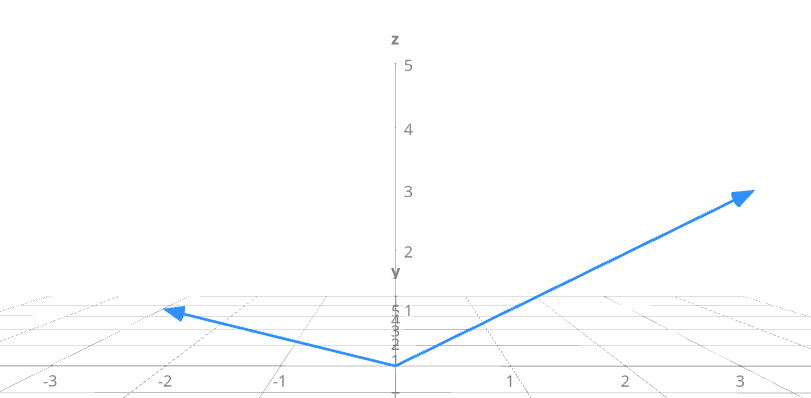
\includegraphics[width=1\textwidth]{examples/1-1.png} 
                \caption{Geometric representation of 2D Vectors.}
                \label{fig:1}
            \end{figure}
        
            Geometrically, a vector can be visualized as an arrow going from the origin to a point.
            Example:
            \begin{equation}
                \vec{v}_1 = \begin{bmatrix} 3 \\ 3 \end{bmatrix}  
                \vec{v}_2 = \begin{bmatrix} -2 \\ 1 \end{bmatrix}
            \end{equation}
            
            \begin{figure}[H]
                \centering
                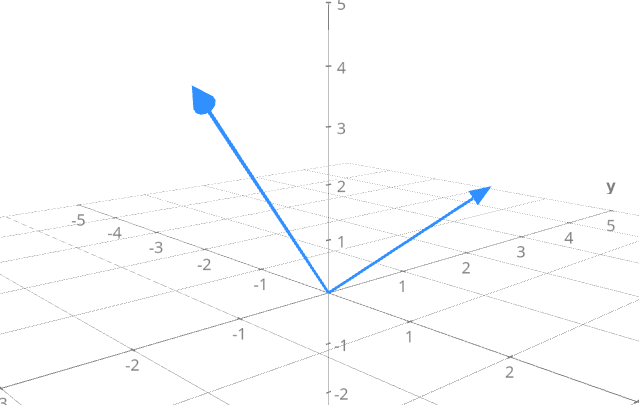
\includegraphics[width=1\textwidth]{examples/1-2.png} 
                \caption{Geometric representation of 3D Vectors.}
                \label{fig:2}
            \end{figure}
            
            The same principle works with a 3D vector but pointing to ($x, y, z$) \\
            Example:
            \begin{equation}
                \vec{v}_1 = \begin{bmatrix} 1 \\ 1 \\ 2 \end{bmatrix}
                \vec{v}_2 = \begin{bmatrix} 1 \\ -2 \\ 4 \end{bmatrix}
            \end{equation}

            Geometrically, vectors can also be thought of as the sum of scalar multiples of the \emph{unit vectors}: $\ihat = \begin{bmatrix}
                1 \\ 0 \\ 0
            \end{bmatrix}$, $\jhat = \begin{bmatrix}
                0 \\ 1 \\ 0
            \end{bmatrix}$, and $\khat = \begin{bmatrix}
                0 \\ 0 \\ 1
            \end{bmatrix}$.

            A vector $\vec{v} = \begin{bmatrix}
                2 \\ -3
            \end{bmatrix}$ can also be written as $\vec{v} = 2\ihat - 3\jhat$

        \subsubsection{Programmatically}
            In Computer Science, common usages of vectors can be:
            \begin{itemize}
                \item A list/array
                \item Method to represent states (e.g., pixel colors, probability, features in ML)
                \item A direction in computer graphics/physics
                \item A velocity or force
                \item Rotation
            \end{itemize}

            \begin{example}[C++ Representation] 
            Here is an example script using the `vector` class of the C++ standard library.
            \begin{lstlisting}[language=C++]
#include <iostream>
#include <vector>

int main() {
    std::vector<int> v1 = {3, 4};
    std::vector<int> v2 = {-2, 1};

    std::vector<int> sum(2);
    for (size_t i = 0; i < 2; ++i) {
        sum[i] = v1[i] + v2[i];
    }

    std::cout << "v1 + v2 = [";
    for (size_t i = 0; i < 2; ++i) {
        std::cout << sum[i];
        f (i < 1) std::cout << ", ";
    }
    std::cout << "]" << std::endl;
    return 0;
}
            \end{lstlisting}
            \end{example}
    \section{Vector Operations}
        \subsection{Magnitude}
            The magnitude of a vector $\vec{v}$, written as $\| \vec{v} \|$, is simply the square root of the squares of each of its elements.
            \begin{equation}
                ||\vec{v}|| = \sqrt{v^2_1 + v^2_2 \cdot\cdot\cdot + v^2_n}
            \end{equation}

            Example:
            \begin{equation}
                ||\begin{bmatrix} 3 \\ 4 \end{bmatrix}|| = \sqrt{3^2 + 4^2} = 5
            \end{equation}

            \emph{Note}: The letter $n$ is commonly used to denote the length of a vector, which is the amount of elements it contains. \\
            Also worth noting: A unit vector is a vector with a magnitude of 1.
    
        \subsection{Vector Addition}
            If both vectors are the same length, you can combine 2 vectors by adding their \emph{components}.
            \begin{equation}
                \vec{a + b} =
                    \begin{bmatrix} a_1 \\ a_2 \\ \cdot \\ \cdot \\ \cdot \\ a_n \end{bmatrix} +
                    \begin{bmatrix} b_1 \\ b_2 \\ \cdot \\ \cdot \\ \cdot \\ b_n \end{bmatrix} =
                    \begin{bmatrix} a_1 + b_2 \\ a_2 + b_2 \\ \cdot \\ \cdot \\ \cdot \\ a_n + a_b \end{bmatrix}
            \end{equation}

            Example:
            \begin{equation}
                \vec{a + b} =
                    \begin{bmatrix} 1 \\ 2 \\ 3 \\ 4 \end{bmatrix} +
                    \begin{bmatrix} 5 \\ 6 \\ 7 \\ 8 \end{bmatrix} =
                    \begin{bmatrix} 6 \\ 8 \\ 10 \\ 12 \end{bmatrix}
            \end{equation}

        \subsection{Vector Subtraction}
            If both vectors are the same length, you can subtract 2 vectors by subtracting their \emph{components}.
            \begin{equation}
                \vec{a - b} =
                    \begin{bmatrix} a_1 \\ a_2 \\ \cdot \\ \cdot \\ \cdot \\ a_n \end{bmatrix} -
                    \begin{bmatrix} b_1 \\ b_2 \\ \cdot \\ \cdot \\ \cdot \\ b_n \end{bmatrix} =
                    \begin{bmatrix} a_1 - b_2 \\ a_2 - b_2 \\ \cdot \\ \cdot \\ \cdot \\ a_n - a_b \end{bmatrix}
            \end{equation}

            Example:
            \begin{equation}
                \vec{a - b} =
                    \begin{bmatrix} 5 \\ 6 \\ 7 \\ 8 \end{bmatrix} -
                    \begin{bmatrix} 1 \\ 2 \\ 3 \\ 4 \end{bmatrix} =
                    \begin{bmatrix} 4 \\ 4 \\ 4 \\ 4 \end{bmatrix}
            \end{equation}

        \newpage
        \subsection{Scalar Multiplication}
            Scalar multiplication is the act of multiplying a vector by a scalar. You multiply the scalar to all \emph{components} inside the vector.

            \begin{equation}
                c \cdot \vec{a} = c \cdot
                    \begin{bmatrix} a_1 \\ a_2 \\ \cdot \\ \cdot \\ \cdot \\ a_n \end{bmatrix} =
                    \begin{bmatrix}  c \cdot a_1 \\ c \cdot a_2 \\ \cdot \\ \cdot \\ \cdot \\  c \cdot a_n \end{bmatrix} 
                \text{where } c \in \mathbb{R}
            \end{equation}

            Example:
            \begin{equation}
                5 \cdot \begin{bmatrix} 1 \\ 2 \\ 3 \\ 4 \end{bmatrix} =
                \begin{bmatrix} 5 \\ 10 \\ 15 \\ 20 \end{bmatrix}
            \end{equation}

        \subsection{Dot Product}
            The dot product (also known as the \emph{inner product} is the sum of all components between two vectors.

            Algebraically it can be used to measure the similarity between 2 vectors.
            If you have 2 vectors of the same size:

            \begin{equation}
                \vec{u} = \begin{bmatrix} u_1 \\ u_2 \\ \cdot \\ \cdot \\ \cdot \\ u_n \end{bmatrix},
                \vec{v} = \begin{bmatrix} v_1 \\ v_2 \\ \cdot \\ \cdot \\ \cdot \\ v_n \end{bmatrix} 
            \end{equation}

            Then the \textbf{dot product} would be:

            \begin{equation}
                \vec{u} \cdot \vec{v} = u_1v_1 + u_2v_2 +\cdot \cdot \cdot + u_nv_n
            \end{equation}

            \newpage
            Example:

            \begin{equation}
                \vec{u} = \begin{bmatrix} 2 \\ 3 \end{bmatrix},
                \vec{v} = \begin{bmatrix} 4 \\ -1 \end{bmatrix}
            \end{equation}

            \begin{equation}
                \vec{u} \cdot \vec{v} = (2 \cdot 4) + (4 \cdot -1) = 8 -3 = 5
            \end{equation}

            The dot product can also relate to angles between vectors:

            \begin{equation}
                \vec{u} \cdot \vec{v} = \|\vec{u}\| \|\vec{v}\|\\cos\theta
            \end{equation}

            \begin{itemize}
                \item $\|\vec{u}\|$ is the magnitude (length) of $\vec{u}$
                \item $\theta$ is the angle between $\|\vec{u}\|$ and $\|\vec{v}\|$
            \end{itemize}

            Useful notes:

            \begin{itemize}
                \item If $\vec{u} \cdot \vec{v}$ 
                    > 0: Vectors are pointing in a similar direction.
                \item If $\vec{u} \cdot \vec{v}$ 
                    < 0: vectors are pointing in opposite directions.
                \item If $\vec{u} \cdot \vec{v}$ 
                    = 0: vectors are perpendicular
            \end{itemize}

        \subsection{Cross Product}
            The cross product of two vectors is another vector that is perpendicular to both factors.

            \begin{equation}
                \vec{u} \times \vec{v} = \begin{bmatrix} a_2b_3 - a_3b_2 \\ a_3b_1 - a_1b_3 \\ a_1b_2 - a_2b_1 \end{bmatrix}
            \end{equation}

        \subsection{Normalization}
            Normalization converts a vector into a \emph{unit vector}.

            \begin{equation}
                \hat{a} = \frac{\vec{a}}{||\vec{a}||}
            \end{equation}

            When a vector is \emph{hatted} (e.g., $\hat{a}, \hat{b}$), it is a unit vector.
\end{document}
